\documentclass[../../course]{subfiles}

\renewcommand\thesection{\arabic{section}}


\begin{document}

\section{Generating Sequences} \label{sec:wrkGeneratingSeqcuences}

First of all we need to generate these three sequences, with frequences of:

\begin{align}
    f_{1} &= 28 \si{Hz}                         \label{eqn:freq1} \\
    f_{2} &= 2 \times 28         = 56   \si{Hz} \label{eqn:freq2} \\
    f_{3} &= (2 \times 28) + 0.1 = 56.1 \si{Hz} \label{eqn:freq3}
\end{align}

Now we need to decide whether we need to generate a \emph{sine} signal or one with
$90 \degree$ phase shift, ie, the \emph{cosine} signal. If we mix\footnote{like, real
part and imaginary part having a phase difference} \emph{sine} and \emph{cosine} we may
get a different kind of \emph{complex} sequence than if we mix \emph{sine} to \emph{sine}
or \emph{cosine} to \emph{cosine}. For our analysis, let's stick with having zero phase
shift between the signals that we are mixing. So let's just mix \emph{sine} signals with
the above frequencies.


To get the continous feel of these sequences let's generate them with $1000$ samples.
And these signals will range from $0$ to $\frac{\pi}{4}$.


Therefore these signals will be:

\begin{itemize} [label=]
    \item
        \begin{align}
            x_{1}(t) =
            \begin{cases}
                \sin(2 \pi 28 t) & \text{; for} \; 0 \le t \le \dfrac{\pi}{4}
            \end{cases}
        \end{align}

    \item
        \begin{align}
            x_{2}(t) =
            \begin{cases}
                \sin(2 \pi 56 t) & \text{; for} \; 0 \le t \le \dfrac{\pi}{4}
            \end{cases}
        \end{align}

    \item
        \begin{align}
            x_{3}(t) =
            \begin{cases}
                \sin(2 \pi 56.1 t) & \text{; for} \; 0 \le t \le \dfrac{\pi}{4}
            \end{cases}
        \end{align}

\end{itemize}

\subsection{Python Implementation}

%python/three_sequences.py%
\begin{minted}[breaklines, autogobble, mathescape] {python}
    import numpy as np
    import pandas as pd

    F = 28
    t = np.linspace(0, np.pi / 4, 1000)

    x1 = np.sin( 2 * np.pi * F * t)
    x2 = np.sin( 2 * np.pi * 2 * F * t)
    x3 = np.sin( 2 * np.pi * (2 * F + 0.1) * t)

    data = pd.DataFrame(
        {
            "x1": x1,
            "x2": x2,
            "x3": x3,
        }
    )

    data.to_csv("../data/three_sequences.csv", sep = " ", index_label = "time")
    print(data)

\end{minted}

\paragraph{Output}

\begin{minted}[breaklines, autogobble] {text}
               x1        x2        x3
    0    0.000000  0.000000  0.000000
    1    0.137872  0.273111  0.273586
    2    0.273111  0.525456  0.526296
    3    0.403133  0.737848  0.738848
    4    0.525456  0.894138  0.895021
    ..        ...       ...       ...
    995 -0.571938 -0.938318 -0.664054
    996 -0.453380 -0.808210 -0.434163
    997 -0.326162 -0.616651 -0.171142
    998 -0.192715 -0.378204  0.104937
    999 -0.055586 -0.111001  0.373009

    [1000 rows x 3 columns]
\end{minted}

\subsubsection{Plots}

\begin{figure} [H]
    \centering
    \adjustbox{max width = \textwidth} {
        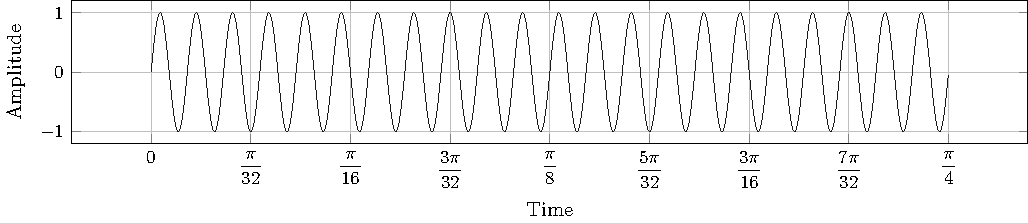
\includegraphics[height = 0.8\textheight] {tikzpics/plotSeqX1.pdf}
    }
    \captionof{figure} {Sine signal with frequency 28}
    \label{plt:seqx1}
\end{figure}

\begin{figure} [H]
    \centering
    \adjustbox{max width = \textwidth} {
        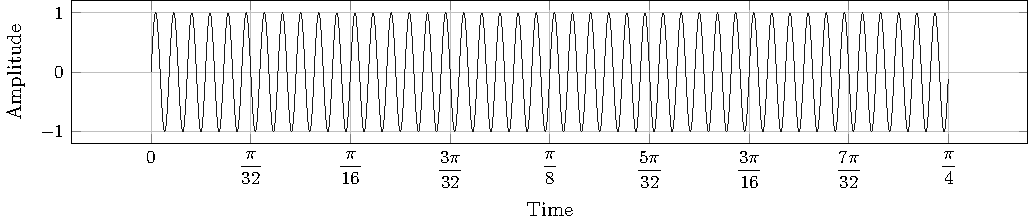
\includegraphics[height = 0.8\textheight] {tikzpics/plotSeqX2.pdf}
    }
    \captionof{figure} {Sine signal with frequency 56}
    \label{plt:seqx2}
\end{figure}

\begin{figure} [H]
    \centering
    \adjustbox{max width = \textwidth} {
        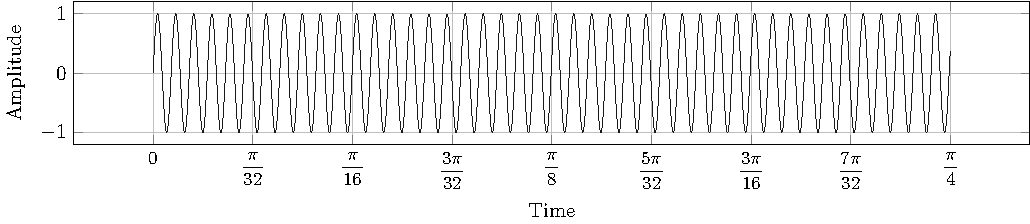
\includegraphics[height = 0.8\textheight] {tikzpics/plotSeqX3.pdf}
    }
    \captionof{figure} {Sine signal with frequency 56.1}
    \label{plt:seqx3}
\end{figure}

\end{document}
